\documentclass[border=5pt]{standalone}
\usepackage{tikz}
\usepackage{tikz-3dplot}
\usetikzlibrary{arrows.meta, 3d, perspective, calc, matrix, positioning}
\usepackage{amsmath}
\begin{document}
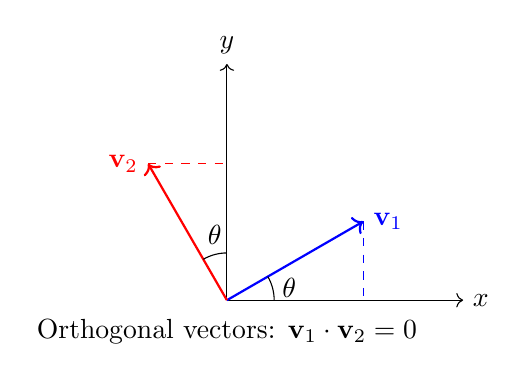
\begin{tikzpicture}[scale=2]
    % Coordinate axes
    \draw[->] (0,0) -- (1.5,0) node[right] {$x$};
    \draw[->] (0,0) -- (0,1.5) node[above] {$y$};

    % Draw orthogonal vectors
    \draw[->, thick, blue] (0,0) -- (0.866,0.5) node[right] {$\mathbf{v}_1$};
    \draw[->, thick, red] (0,0) -- (-0.5,0.866) node[left] {$\mathbf{v}_2$};

    % Show they're orthogonal
    \draw[dashed, blue] (0.866,0.5) -- (0.866,0);
    \draw[dashed, red] (-0.5,0.866) -- (0,0.866);

    % Angle
    \draw (0.3,0) arc (0:30:0.3) node[right, midway] at (0.2,0.15) {$\theta$};
    \draw (0,0.3) arc (90:120:0.3) node[above, midway] at (-0.15,0.2) {$\theta$};

    \node at (0,-0.2) {Orthogonal vectors: $\mathbf{v}_1 \cdot \mathbf{v}_2 = 0$};
\end{tikzpicture}
\end{document}
